\documentclass{article}
\usepackage{import}
\usepackage{../style/header}
\def\module{MATH40005A Probability}
\def\lecturer{Professor Almut Veraart}
\def\term{Autumn 2023}
\def\cover{ 
$$
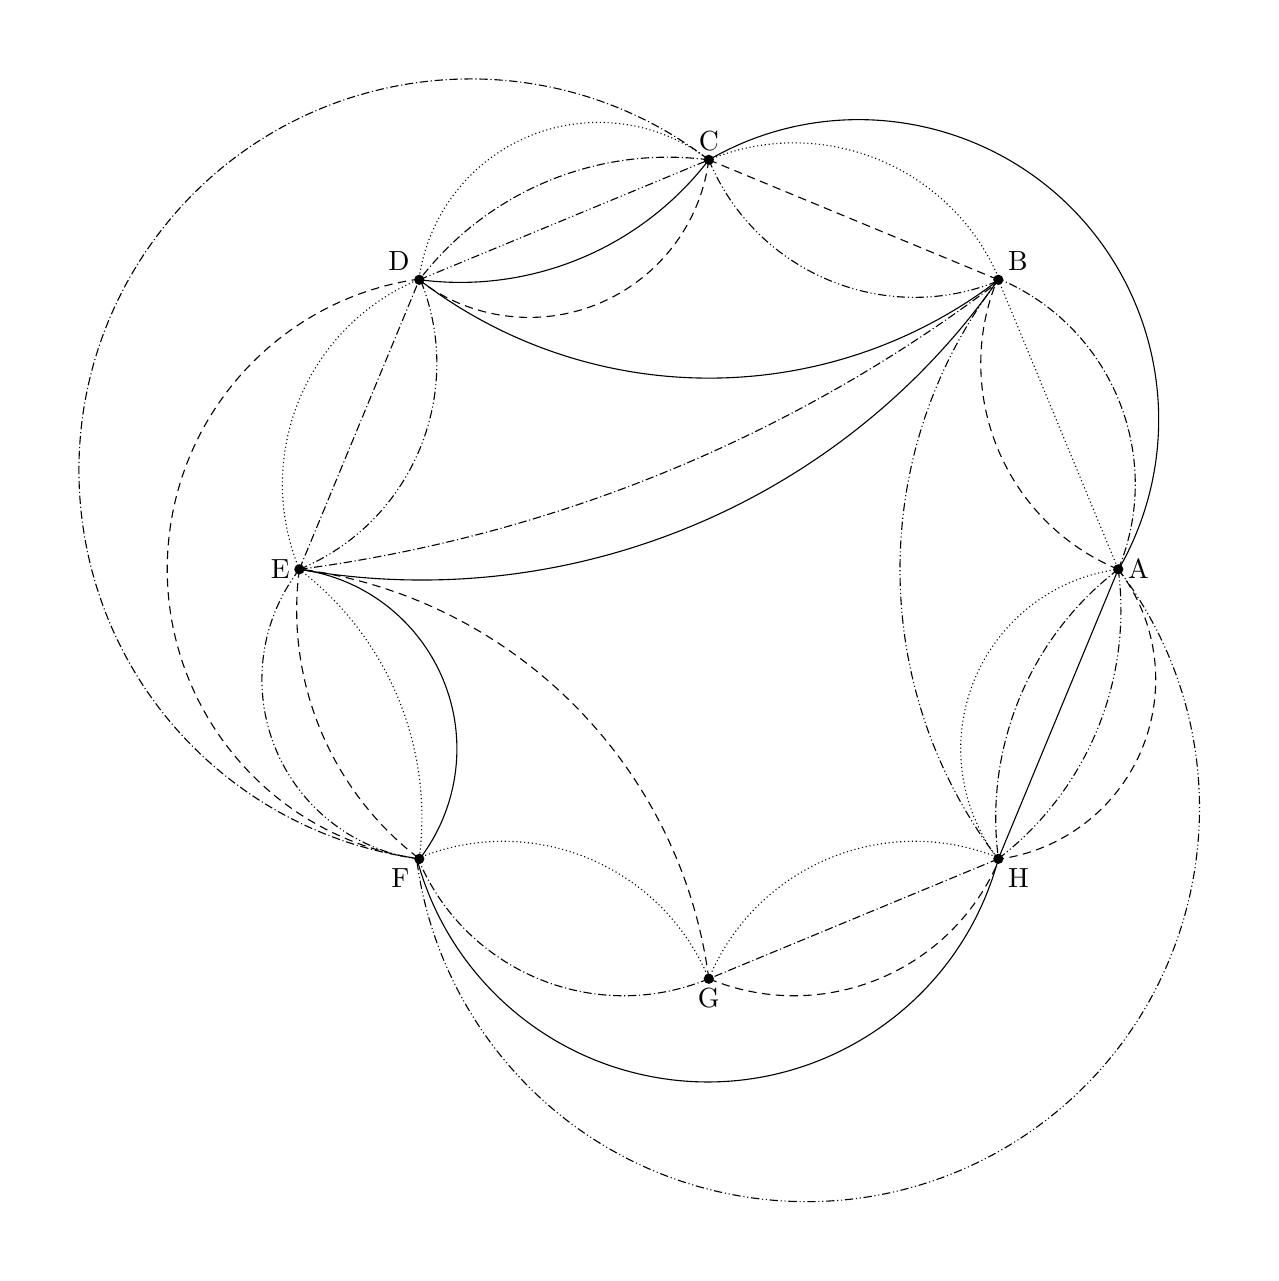
\begin{tikzpicture}[scale=1.3]
    \draw[black] (4,0) -- ({2*sqrt(2)},{-2*sqrt(2)});
    \draw[black] (0,4) arc (-37.5:-97.5:3.06);
    \draw[black] (-4,0) arc (82.5:-37.5:1.77);
    \draw[black] (0,4) arc (120:-30:2.93);
    \draw[black] ({2*sqrt(2)},{-2*sqrt(2)}) arc (-15:-165:2.94);
    \draw[black] ({-2*sqrt(2)},{2*sqrt(2)}) arc (232.5:307.5:4.65);
    \draw[black] (-4,0) arc (-100:-34.8:6.875);
    
    \draw[black, densely dotted] ({2*sqrt(2)},{2*sqrt(2)}) -- (4,0);
    \draw[black, densely dotted] (-4,0) arc (52.5:-7.5:3.06);
    \draw[black, densely dotted] (0,4) arc (112.5:22.5:2.175);
    \draw[black, densely dotted] (0,-4) arc (22.5:112.5:2.175);
    \draw[black, densely dotted] (0,-4) arc (157.5:67.5:2.175);
    \draw[black, densely dotted] (-4,0) arc(202.5:112.5:2.17);
    \draw[black, densely dotted] (0,4) arc (52.5:172.5:1.77);
    \draw[black, densely dotted] (4,0) arc (97.5:217.5:1.77);
    
    \draw[black, densely dashed] (0,4) -- ({2*sqrt(2)},{2*sqrt(2)});
    \draw[black, densely dashed] (-4,0) arc (172.5:232.5:3.06);
    \draw[black, densely dashed] (4,0) arc (247.5:157.5:2.175);
    \draw[black, densely dashed] (0,-4) arc (-112.5:-22.5:2.175);
    \draw[black, densely dashed] (4,0) arc (37.5:-82.5:1.77);
    \draw[black, densely dashed] (0,4) arc (-7.5:-127.5:1.77);
    \draw[black, densely dashed] ({-2*sqrt(2)},{-2*sqrt(2)}) arc (-98:-262:2.86);
    \draw[black, densely dashed] (0,-4) arc (7.5:82.5:4.65);
    
    \draw[black, densely dashdotted] ({2*sqrt(2)},{-2*sqrt(2)}) -- (0,-4);
    \draw[black, densely dashdotted] (-4,0) -- ({-2*sqrt(2)},{2*sqrt(2)});
    \draw[black, densely dashdotted] (0,4) arc (82.5:142.5:3.06);
    \draw[black, densely dashdotted] (4,0) arc (127.5:187.5:3.06);
    \draw[black, densely dashdotted] (4,0) arc (-22.5:67.5:2.175);
    \draw[black, densely dashdotted] (0,-4) arc (-67.5:-157.5:2.175);
    \draw[black, densely dashdotted] (0,4) arc (52.5:262.5:3.825);
    \draw[black, densely dashdotted] (-4,0) arc (-82.5:-52.8:14.4);
    
    \draw[black, densely dashdotdotted] ({-2*sqrt(2)},{2*sqrt(2)}) -- (0,4);
    \draw[black, densely dashdotdotted] (4,0) arc (7.5:-52.5:3.06);
    \draw[black, densely dashdotdotted] (0,4) arc (202.5:292.5:2.175);
    \draw[black, densely dashdotdotted] (-4,0) arc (-67.5:22.5:2.175);
    \draw[black, densely dashdotdotted] (-4,0) arc (142.5:262.5:1.77);
    \draw[black, densely dashdotdotted] (4,0) arc (37.5:-172.5:3.84);
    \draw[black, densely dashdotdotted] ({2*sqrt(2)},{2*sqrt(2)}) arc (142.5:217.5:4.65);
    
    \fill (4,0) circle (0.05) node[right]{A};
    \fill ({2*sqrt(2)},{2*sqrt(2)}) circle (0.05) node[above right]{B};
    \fill (0,4) circle (0.05) node[above]{C};
    \fill ({-2*sqrt(2)},{2*sqrt(2)}) circle (0.05) node[above left]{D};
    \fill (-4,0) circle (0.05) node[left]{E};
    \fill ({-2*sqrt(2)},{-2*sqrt(2)}) circle (0.05) node[below left]{F};
    \fill (0,-4) circle (0.05) node[below]{G};
    \fill ({2*sqrt(2)},{-2*sqrt(2)}) circle (0.05) node[below right]{H};
\end{tikzpicture}
$$

\begin{center}
    A minimum vertex 5-Venn diagram.
\end{center}
}
\def\syllabus{Basic set theory and combinatorics, Kolmogorov probability axioms, Conditional probability and independence, DRVs, CRVs, Transformations, Expectaction, Variance, Multivariate calculus, Joint Distributions, LOTUS, pgfs, mgfs, conditional distribution}
\def\thm{subsection}

\begin{document}

% Title page
\maketitle
\cover
\vfill
\begin{abstract}
\noindent\syllabus
\end{abstract}

\pagebreak

% Contents page
\tableofcontents

\pagebreak

% Document page
\setcounter{section}{-1}

\section{Introduction}

\lecture{1}{Monday}{30/10/2023}

The following are complementary reading for the course.
\begin{itemize}
\item G. Grimmett and D. J. A. Welsh, Probability: An Introduction, 1986
\item J. K. Blitzstein and J. Hwang, Introduction to Probability, 2019
\item D. F. Anderson et al, Introduction to Probability, 2018
\item S. M. Ross, Introduction to Pro ability Models, 2014
\item G. Grimmett and D. Stirzaker, Probability and Random Processes, 2001
\item G. Grimmett and D. Stirzaker, One Thousand Exercises in Probability, 2009
\end{itemize}

These notes are written assuming all material covered in ICL's \textbf{MATH40001}, \textbf{MATH40002}, \textbf{MATH40003A} and \textbf{MATH40004}.

\begin{notation*}
    Common notation is all defined precisely in the aforementioned. The controversial and additional things are defined as such: $\NN = \{1,2,3,...\}$, $\NN_0 := \NN \cup \{0\}$, $\RR^{>0} := (0,\infty)$.
\end{notation*}


\subsection{Sample spaces and set theory}

\begin{definition}
    The \textbf{sample space} $\Omega$ is the set of all possible outcomes of an experiment. An element of the sample space $\omega \in \Omega$ is a \textbf{sample point}.
\end{definition}

\begin{examples}
    When flipping a coin $\Omega  = \{H,T\}$. When rolling a standard die $\Omega = \{1,2,3,4,5,6\}$.
\end{examples}

\begin{definition}
    Subsets of $\Omega$ are collections of sample points and called \textbf{events}.
\end{definition}

Suppose events $A,B\subseteq\Omega$:
\begin{itemize}
    \item $A\cup B$ is the event that $A$ or $B$ or both occur,
    \item $A\cap B$ is the event that $A$ and $B$ both occur,
    \item $A^c = \bar{A}$ is the event that occurs iff $A$ does not occur.
\end{itemize}


Let $\III$ be a general index set with $A_i \subseteq\Omega,\; \forall i \in\III$ and $B \subseteq \Omega$. The following identities hold.
\[
\left( \bigcup_{i\in\III}A_i \right)^c = \bigcap_{i\in\III}A_i^c \textcolor{black}{,} \quad
\left( \bigcap_{i\in\III}A_i \right)^c = \bigcup_{i\in\III}A_i^c \textcolor{black}{,} \qquad
B \cap \left( \bigcup_{i\in\III}A_i \right) = \bigcap_{i\in\III}(A_i\cup B) \textcolor{black}{,} \quad
B \cup \left( \bigcap_{i\in\III}A_i \right) = \bigcup_{i\in\III}(A_i\cap B) \textcolor{black}{.}
\]
These are \textbf{De Morgan's Laws} and \textbf{Distributivity} respectively.

\lecture{2}{Tuesday}{31/10/2023}

\subsection{Interpretation of probability}
\begin{definition}
    The \textbf{Cardinality} of a set, denoted $\text{card}(A)$ or $|A|$ is the number of elements in the set $A$.
\end{definition}

\begin{definition}
    Two sets have the same cardinality iff there exists a bijection between the them.
\end{definition}

\begin{definition}
    $A$ is \textbf{finite} if it has as finite numbers of elements, $A$ is \textbf{countably infinite} if there exists a bijection $f: A \to \NN$, $A$ if \textbf{countable} if it is finite or countable infinite, $A$ is \textbf{uncountable} or \textbf{uncountable infinite} if it isn't countable.
\end{definition}

Samples spaces can be countable or uncountable.

\begin{definition}[Naive probability]
    Suppose $|A| < \infty$ and we want to assign a probability to $A \subseteq \Omega$.
    \[
    \P_{Naive}(A) := \frac{|A|}{|\Omega|} \implies \P(A^c) = 1 - \P(A)  \textcolor{black}{.}
    \]
    This Naive example does not consider when $|A|$ is infinite but of finite area.
\end{definition}
\begin{example}
    Let $\Omega = \{(x,y) \in \RR^2, x^2+y^2=1\}$ and $A\subseteq\Omega$. Define: 
    \[
    \P(A) := \frac{\text{area of } A}{\text{area of } \Omega}
    \]
    In the case where $A = \{(x,y) \in \RR^2, x^2+y^2=0.5^2\}$ we have $\P(A) = 0.25$
\end{example}
\begin{remark}
    For classical / naive probability we require $|\Omega| < \infty$ or the ``area" of $\Omega$ be finite. 
\end{remark}


\begin{definition}[Limiting frequency]
    Consider $n_{total}$ repetitions of an experiment and $n_A$ the number of time $A$ occurs.
    \[\P(A) := \lim_{n_{total} \to \infty} \frac{n_A}{n_{total}}\]
    Unfortunately, $n_{total} \to \infty$ is often hard to conceive with finite representations not necessarily being representative.
\end{definition}

\begin{definition}[Subjective probability]
    For an event $A$ assign the probability $\P(A)$ based on our own personal beliefs. The subjective probability need not be the same for different individuals, and despite its appearance it remains a valid interpretation of probability.
\end{definition}

\begin{remark}
    All three interpretations of probability depend of assumptions about the experiment.
\end{remark}

\lecture{3}{Friday}{03/11/2023}

\section{Counting}
\subsection{Multiplication principle}
Computing naive probabilities often requires some combinatorics.

\begin{definition}[Multiplication  principle]
    If we perform an experiment $A$ that has $a$ possible outcomes and an experiment $B$ with $b$ possible outcomes (in any order) then the number of outcomes of the  \textbf{compound experiment} will be $ab$.
\end{definition}

\begin{remark}
    When dealing with repetitions of the same experiment (with sample space $\Omega$, the sample space is given by the Cartesian product of the individual samples spaces.
    \[
        \Omega_1 \times \Omega_2 \times \cdots \times \Omega_n :=  \{(\omega_1,\omega_2,\ldots,\omega_n): \omega_i \in \Omega_i\}\textcolor{black}{.}
    \]
    The cardinality of this samples space follows from the multiplication principle.
\end{remark}

\subsection{Power sets}
\begingroup\belowdisplayskip=-10pt
    \begin{definition}[Power Set]
        Given a set $A$ its \textbf{power set} is defined as:
        \[
            \PPP(A) := \{X:X\subseteq A\}\textcolor{black}{.}
        \]
    \end{definition}
\endgroup

\begin{theorem}
    If $A$ is a finite set, $|\PPP(A)|=2^{|A|}$.
\end{theorem}

\subsection{Combinatorial coefficients}

\begingroup\belowdisplayskip=-0pt
    \begin{definition}[Factorial]
        Let $n\in\NN$ the \textbf{factorial} of $n$ is defined as:
        \[
        n! := \prod_{i=1}^ni\textcolor{black}{.}
        \]
    \end{definition}
\endgroup

\begingroup\belowdisplayskip=-10pt
    \begin{definition}[Descending factorial]
        Let $k,n\in\NN$ with $k\leq n$ the \textbf{descending factorial} denoted $(n)_k$ is defined as:
        \[
        (n)_k := n(n-1)\ldots(n-k+1) = \prod_{i=0}^{k-1}(n-i) = \prod_{j=n-k+1}^{n}j = \frac{n!}{(n-k)!}\textcolor{black}{.}
        \]
    \end{definition}
\endgroup

\begingroup\belowdisplayskip=-10pt
    \begin{definition}[Binomial coefficient]
        Let $k,n\in\NN_0$ the \textbf{binomial coefficient} is the number of subsets of size $k$ of a set $n$:
        \[ 
            \binom{n}{k} := 
            \begin{dcases}
            \frac{n(n-1)\ldots(n-(k-1))}{k!} = \frac{(n)_k}{k!} = \frac{n!}{(n-k)!k!} & \textcolor{black}{\text{if }} k\leq n \\
            \omit\hfil0\hfil & \textcolor{black}{\text{otherwise.}}
            \end{dcases}
        \]
    \end{definition}
\endgroup

\lecture{4}{Monday}{06/11/2023}

\subsection{Sampling with and without replacement}
``Definitions" given in the context of drawing balls from an urn, $S=\{1,2,\ldots,n\}$.
\begin{definition}[Ordered sampling with replacement]
    Take out a ball from $S$, note its number, put it back; repeat this $k$ times. The sample space for this experiment is $\Omega = S^k$.
\end{definition}

\begin{definition}[Ordered sampling without replacement]
    Take out a ball form $S$, note its number but \textbf{do not} put it back; repeat $k<n$ times. There are $|\Omega| = (n)_k$ possible outcomes.
\end{definition}


\begin{definition}[Unordered sampling without replacement]
    We take $k$ balls out of the urn, there are $\binom{n}{k}$ possibilities.
\end{definition}

\begingroup\belowdisplayskip=-10pt
    \begin{definition}[Unordered sampling with replacement]
        We take $k$ balls out of the urn, with the stars and bars argument: there must be $k$ stars divided by $n-1$ bars giving us:
        \[
        |\Omega| = \binom{n+k-1}{k} = \binom{n+k-1}{n-1}\textcolor{black}{.}
        \]
    \end{definition}
\endgroup

\lecture{5}{Tuesday}{07/11/2023}

\section{Axiomatic probability}
\subsection{Event space}
We do not always want to consider all subsets of $\Omega$ so denote $\FFF \subseteq \PPP(\Omega)$ the \textbf{event space}, which contains the events we are allowed to consider. $\FFF$ must always be a $\sigma$-algebra.

\begin{definition}[Algebra]
    $\FFF$ is an \textbf{algebra} (or a field) on $\Omega$ iff:\\
    \begin{enumerate*}
        \item $\emptyset \in \FFF$, \hspace{100pt}
        \item $A \in \FFF \implies A^c \in \FFF$, \hspace{100pt}
        \item $A,B \in \FFF \implies A\cup B \in \FFF$.
    \end{enumerate*}
\end{definition}

\begin{definition}[$\sigma$-algebra]
    $\FFF$ is a \textbf{$\sigma$-algebra} (or a $\sigma$-field) on $\Omega$ iff:\\
    \begin{enumerate*}
        \item $\emptyset \in \FFF$; \hspace{15pt}
        \item $A \in \FFF \implies A^c \in \FFF$, \hspace{15pt}
        \item For all $i$ in some countable indexing set $\III$, $A_i \in \FFF \implies \bigcup\limits_{i\in \III}A_i \in \FFF$.
    \end{enumerate*}
\end{definition}

\begin{remark}
    \begin{enumerate}
        \item Any algebra is closed under finite unions and finite intersections,
        \item Any $\sigma$-algebra is closed under countable intersections,
        \item Any ($\sigma$-)algebra on $\Omega$ contains $\Omega$.
    \end{enumerate}
\end{remark}

\begin{definition}[Trivial sigma algebra]
    The \textbf{trivial sigma algebra} on $\Omega$ is defined as $\FFF_{trivial} := \{ \emptyset, \Omega \}$.
\end{definition}

\begin{example}[Smallest $\sigma$-algebra of an element]
    For some $A \subseteq \Omega$, the sigma algebra $\FFF_A := \{\emptyset, A, A^c , \Omega \}$ is the smallest $\sigma$-algebra on $\Omega$ (smallest cardinality) that contains $A$.
\end{example}

\lecture{6}{Friday}{10/11/2023}

\subsection{Probability measure}

\begingroup\belowdisplayskip=-10pt
    \begin{definition}[Probability measure]
        A mapping $\P: \FFF \to \RR$ is a \textbf{probability measure} on $(\Omega, \FFF)$ iff:\\
        \begin{enumerate*}
            \item $\P(A)\geq0$ for all $A\in\FFF$;
            \item $\P(\Omega) = 1$;
            \item for a countable, disjoint sequence of events $(A_i)_{i\in\III}$ on an indexing set $\III$: \\
        \end{enumerate*}
        \[
        \P\left(\bigcup_{i\in\III}A_i\right) = \sum_{i\in\III}\P(A_i)\textcolor{black}{.}
        \]
    \end{definition}
\endgroup

\begingroup\abovedisplayskip=-10pt 
\subsection{Probability space}
\endgroup
\begin{definition}[Probability space]
    A \textbf{probability space} is a triple $(\Omega, \FFF, \P)$, with $\Omega$ a sample space, $\FFF$ a $\sigma$-algebra on $\Omega$, and $\P$ a probability measure on $(\Omega, \FFF)$.
\end{definition}

\begin{corollary} For $A,B \in \FFF$: \newline
    \begin{enumerate*}
        \item $\P(A^c) = 1 - \P(A)$, \hspace{25pt}
        \item $A \subseteq B \implies \P(A) \leq \P(B)$, \hspace{25pt}
        \item $\P(A\cup B) = \P(A) + \P(B) - \P(A\cap B)$.
    \end{enumerate*}
\end{corollary}

\lecture{7}{Monday}{13/11/2023}
\section{Conditional probability}
\begin{definition}[Conditional probability measure]
    Consider the probability space $(\Omega, \FFF, \P)$ and some event $B \in \FFF$ with $\P(B) > 0$, we construct the probability measure $\Q$ on $(\Omega, \FFF)$ by \[
        \Q(A):=\frac{P(A\cap B)}{P(B)}\textcolor{black}{.}
    \]
    Denote the \textbf{conditional probability} of $A$ given $B$ by $P(A|B) = Q(B)$.
\end{definition}

\lecture{8}{Tuesday}{14/11/2023}
\subsection{Bayes' rule and total probability}

\begingroup\belowdisplayskip=-10pt
\begin{theorem}[Bayes' rule]
    For $A,B \in \FFF$ with $\P(A) >0, \P(B) > 0$ we have, \[
        \P(A|B) = \frac{\P(B|A)\P(A)}{\P(B)}
        \textcolor{black}{.}
        \]
\end{theorem}
\endgroup

\begin{definition}[Partition of a set]
    A partition of some set $\Omega$ is a collection $\{B_i, i \in \III\}$ for some countable index set $\III$ with $B_i \cap B_j = \emptyset$ for all $i,j\in\III$ with $i\neq j$ and $\bigcup\limits_{i\in\III}B_i = \Omega$.
\end{definition}

\begingroup\belowdisplayskip=-10pt
\begin{theorem}[Total probability]
    Given some partition $\{B_i, i\in\III\}$ of $\Omega$ with $\P(B_i)>0$ for all $i\in\III$ and some event $A\in\FFF$,\[
        \P(A)=\sum_{i\in\III}\P(A\cap B_i)=\sum_{i\in\III}\P(A|B_i)\P(B_i)\textcolor{black}{.}
    \]
\end{theorem}
\endgroup

These two theorems can then be combined to form the following.
\begingroup\belowdisplayskip=-10pt
\begin{theorem}[Bayes' rule with extra conditioning]
    For events $A,B,E \in \FFF$ with $\P(A\cap E)>0, P(B\cap E) > 0$ we have \[
    \P(A|B\cap E) = \frac{\P(B|A\cap E)\P(A|E)}{\P(B|E)}
    \textcolor{black}{.}
    \]
\end{theorem}
\endgroup

\begingroup\belowdisplayskip=-10pt
\begin{theorem}[Total probability with extra conditioning]
    Given events $A,E\in\III$  with $\P(E)>0$ and some partition $\{B_i, i\in\III\}$ of $\Omega$ with $\P(B_i\cap E)>0$ for all $i\in\III$,
    \[
        \P(A|E)=\sum_{i\in\III}\frac{\P(A\cap B_i\cap E)}{\P(E)}
        =\sum_{i\in\III}\P(A|B_i\cap E)\P(B_i| E)
        \textcolor{black}{.}
    \]
\end{theorem}
\endgroup

\lecture{9}{Friday}{17/11/2023}
\section{Independence}
\subsection{Event independence}
Two events $A,B\in\FFF$ will be independent iff the occurrence of one does not effect the probability the other occurs, i.e $\P(A|B) = \P(A)$ and vice versa.

\begin{definition}[Independent events]
    Two events $A,B \in \FFF$ are said to be \textbf{independent} iff\[
    \P(A\cap B) = \P(A)\P(B) \textcolor{black}{,}
    \] and \textbf{dependent} otherwise.
\end{definition}

\begin{corollary}
    If $A$ and $B$ are independent then so are all pairs of their complements.
\end{corollary}

\begin{definition}[General independence]
    A finite collection of events $\{A_1,A_2,\ldots ,A_n\}$ is independent iff \[
    \P(A_1\cap A_2\cap \ldots \cap A_n) = \P(A_1)\P(A_2)\ldots \P(A_n)\textcolor{black}{,}
    \]
    and similarly a countably or uncountably infinite collection of events is independent iff each finite subcollection is independent.
\end{definition}

\lecture{10}{Monday}{20/11/2023}
\subsection{Conditional independence}

\begingroup\belowdisplayskip=-20pt
\begin{definition}[Conditional independence]
    Given the events $A,B,C \in \FFF$ with $\P(C)>0$ we say $A$ and $B$ are \textbf{conditional independent} given $C$ iff, \[
        \P(A\cap B|C) = \P(A|C)\P(B|C) \textcolor{black}{.}
    \]
\end{definition}
\endgroup

\subsection{Product rule for general independence}
The upcoming subsection may seem disparate, they are however necessary parts to the omitted proof of the product rule for general independence and therefore deemed relevant.
\begin{definition}[Set difference]
        Given two set $A,B\in\Omega$ the \textbf{set difference} of $A$ and $B$ is defined as, $A\setminus B := A \cap B^c$.
\end{definition}

\begin{lemma}
    Any countable union of sets can be written as a countable union of disjoint sets.
\end{lemma}

\begin{definition}[Increasing and decreasing sets]
    A sequence of sets $(A_i)_{i=1}^\infty$ is said to \textbf{increase} to $A$ (written $A_i \uparrow A$) iff $A_1 \subseteq A_2 \subseteq \ldots$ and $\bigcup\limits_{i=1}^\infty = A$. The definition for a sequence of sets $(B_i)_{i=1}^\infty$ to \textbf{decrease} to a set $B$ ($B_1 \downarrow B$) is defined similarly.
\end{definition}

\begingroup\belowdisplayskip=-10pt
\begin{theorem}[Continuity property of probability measures]
    If $A_1, A_2, \ldots \in \FFF$ with $A_i \uparrow A$ or $A_i \downarrow A$ for some $A \in \FFF$, \[
        \lim_{i\rightarrow\infty}\P(A_i) = \P(\lim_{i\rightarrow\infty}A_i) = \P(A)
    \textcolor{black}{.}\]
\end{theorem}
\endgroup

\begingroup\belowdisplayskip=-20pt\abovedisplayskip=-10pt
\begin{theorem}[Product rule for general independence]
    Given a countably infinite set of independent events $A_1, A_2, \ldots \in \FFF$, \[
     \P\left(\bigcap_{i=1}^\infty{A_i}\right) = \prod_{i=1}^\infty\P(A_i)\textcolor{black}{.}
    \]
\end{theorem}
\endgroup

\section{Discrete random variables}
\lecture{11}{Tuesday}{21/11/2023}
\subsection{Images and their properties}
throughout this subsection we will be considering the function $f:\XXX \rightarrow \YYY$.
\begin{definition}[Image]
    For some subset $A \subseteq \XXX$ we define the \textbf{image} of $A$ under $f$ by, \[
        f(A) := \{y \in \YYY: \exists x \in A, y = f(x)\} = \{f(x): x \in A\} \textcolor{black}{.}
    \]
When $A = \XXX$, $f(\XXX) = \im f$.
\end{definition}

\begin{definition}[Pre-image]
    For some subset $B \subseteq \YYY$ we now define the \textbf{pre-image} of $B$ under $f$ by, \[
    f^{-1}(B) := \{x\in\XXX: f(x) \in B\} \textcolor{black}{.}
    \]
Despite the similar notation to the inverse function of $f$ they are not the same thing. Notably, the pre-image under $f$ always exists while the inverse function need not exist.
\end{definition}

\begingroup\belowdisplayskip=-10pt
\begin{lemma}
    For a collection of subsets $B_i \in \FFF$ for $i$ in some indexing set $\III$ we have, \[
        f^{-1}\left(\bigcup_{i\in\III} B_i \right) = \bigcup_{i\in\III} f(B_i) \textcolor{black}{.}
    \]
\end{lemma}
\endgroup

\subsection{DRVs and their distributions}

\begin{definition}[Discrete random variable]
    A \textbf{discrete random variable} (\textbf{DRV}) on the probability space $(\Omega, \FFF, \P)$ is a function $X: \Omega \rightarrow \RR$ that satisfies the following properties:
    \begin{itemize}
        \item $\im X = \{X(\omega): \omega \in \Omega\}$ must be a countable subset of $\RR$,
        \item $X^{-1}(x) \in \FFF$ for all $x \in \RR$.
    \end{itemize}
\end{definition}

\begin{remark}
    The nomenclature of $X$ being discrete stems from the fact that its image is a countable subset of $\RR$ and so can be mapped to $\NN$ which we see as being discrete.
\end{remark}

\begin{definition}[Probability mass function]
    The \textbf{probability mass function} (\textbf{pmf}) of a DRV $X$ is defined as a function $p_X: \RR \rightarrow [0,1]$ such that, \[
        p_X(x) := \P(X^{-1}(x))\textcolor{black}{.}
    \]
    This is commonly denoted by $p_X(x) = \P(X=x)$.
\end{definition}

\begin{remark}
    Some useful propoerties of the pmf extending from the definition are:
    \begin{itemize}
        \item $x \not\in \im X \implies p_X(x) = 0$,
        \item For $x_1, x_2 \in \im X$ with $x_1 \neq x_2$, $X^{-1}(x_1) \cap X^{-1}(x_2) = \emptyset$,
        \item $\sum\limits_{x\in\im X}p_X(x) = \sum\limits_{x\in\RR}p_X(x) = 1$.
    \end{itemize}
\end{remark}

\begin{theorem}
    Suppose $\III$ is some indexing set and $S = \{s_i \in \RR: i\in\III\}$ is countable and $\{\pi_i:\i \in \III\}$ is a collection such that $\pi_i \geq 0$ for all $i \in \III$ and $\sum\limits_{i\in\III}\pi_i = 1$. Then there exists some probability space $(\Omega,\FFF,\P)$ and a DRV $X$ on said probability space such that $p_X(s_i)=\pi_i$ for all $i\in\III$ and $p_X(s)=0$ otherwise.
\end{theorem}

\section{Common DRVs}
All DRVs within this section will be considered over the probability space $(\Omega, \FFF, \P)$.
\subsection{Bernoulli distribution}
\begin{definition}[Bernoulli distribution]
    A DRV $X$ is said to have \textbf{Bernoulli distribtuion} with parameter $p\in(0,1)$ if $\im X = \{0,1\}$ with $p_X(1)=p$. This is denoted by $X \sim \text{Bern}(p)$.
\end{definition}

\begingroup\belowdisplayskip = -10pt
\begin{definition}[Indicator variable]
    Given some event $A\in\FFF$ the \textbf{indicator variable} of the event $A$ is given by,\[
    \II_A(\omega) := \begin{dcases}
        1 & \text{\textcolor{black}{if }} \omega \in A \\
        0 & \text{\textcolor{black}{if }} \omega \not\in A
    \end{dcases}
    \textcolor{black}{.}
    \]
\end{definition}
\endgroup

\begin{remark}
    $\II_A \sim \text{Bern}(\P(A))$.
\end{remark}

\subsection{Binomial distribution}
\begin{definition}[Binomial distribution]
    Consider a sequence of $n\in\NN$ iid Bernoulli trials with parameter $p$, count the number of successes and denote this by the random variable $X$ then $\im X = [0,n]$ and, \[p_X(x) = \binom{n}{x}p^x(1-p)^{n-x} \quad \text{\textcolor{black}{for }$x\in[0,n]$}\textcolor{black}{.}\]
We say $X$ follows a \textbf{binomial distribution} and this is denoted by $X \sim \text{Bin}(n,p)$.
\end{definition}

\subsection{Hypergeometric distribution}
As we have done previously, consider of urn of $N\in\NN$ balls with $K\in\NN$ of these being white and the remainder being black from which we will draw $n\in\NN$ balls and want to consider the DRV ($X$) for the number of white balls drawn. When drawing with replacement we have $X \sim \text{Bin}(n,K/N)$. However, when drawing without replacement X follows the hypergeometric distribution.

\begingroup\belowdisplayskip=0pt
\begin{definition}[Hypergeometric distribution]
    A DRV $X$ follows the \textbf{hypergeometric distribution} with three parameters $N\in\NN_0, K\in\NN,n\in[0,N]$ if $\im X = [0,\text{min}(n,K)]$ and, \[
        p_X(x) = \frac{\binom{K}{x}\binom{N-K}{n-x}}{\binom{N}{n}} \quad \text{\textcolor{black}{for }$x\in[0,K]$}\textcolor{black}{.}
    \]
\end{definition}
\endgroup

\begingroup\belowdisplayskip=-10pt
\begin{lemma}[Vandemonde's identity]
    \textbf{Vandemonde's identity} is an important tool in the derivation of the pmf for the hypergeometric distribution and so is included here. The identity is as follows, for $k,m,n \in \NN$ with $k\leq m+n$, we have:
     \[
        \binom{m+n}{k} = \sum_{i=0}^k\binom{m}{i}\binom{n}{k-i}\textcolor{black}{.}
     \]
\end{lemma}
\endgroup

\subsection{Discrete uniform distribution}
\begingroup\belowdisplayskip=-10pt
\begin{definition}[Discrete uniform distribution]
    A DRV $X$ follows the \textbf{discrete uniform distribution} over a nonempty set of numbers $C$, denoted $X \sim \text{DUnif}(C)$, if $\im X = C$ and,
    \[
        p_X(x)=
        \begin{dcases}
            \frac{1}{\text{card}(C)} & \text{\textcolor{black}{for }$x\in C$} \\
            \omit\hfil0\hfil & \text{\textcolor{black}{otherwise}}
        \end{dcases}\textcolor{black}{.}
    \]
\end{definition}
\endgroup

\subsection{Poisson distribution}
The poisson distribution is commonly used for modelling the number of events occurring in a certain time period. Its pdf is derived by taking the $\lim\limits_{n\rightarrow\infty}p_X(x)$ where $X \sim \text{Bin}(n,\frac{\lambda}{n})$ for some $\lambda \in \RR$.

\begingroup\belowdisplayskip=-10pt
\begin{definition}[Poisson distribution]
    A DRV $X$ follows the \textbf{poisson distribution} with parameter $\lambda\in\RR^{>0}$, denoted $X \sim \text{Poi}(\lambda)$, if $\im X = \NN_0$ and, \[
        p_X(x) = \frac{\lambda^x}{x!}e^{-\lambda} \quad \text{\textcolor{black}{for }$x\in\NN_0$}\textcolor{black}{.}
    \]
\end{definition}
\endgroup

\subsection{Geometric distribution}
\begin{definition}[Geometric distribution]
    A DRV $X$ follows the \textbf{geometric distribution} with parameter $p \in (0,1)$, denoted $X \sim \text{Geom}(p)$, if $\im X = \NN$ and, \[
        p_X(x) = (1-p)^xp \quad \text{\textcolor{black}{for }$x\in\NN$}\textcolor{black}{.}
    \]
This can be seen as counting the number of Bernoulli trials with parameter $p$ that occur before a failure.
\end{definition}

\subsection{Negative binomial distribution}
\begingroup\belowdisplayskip=-20pt
\begin{definition}[Generalised binomial coefficient]
    Let $\alpha\in\CC$ and $k\in\NN$ and define the \textbf{generalised binomial coefficient} by,\[
    \binom{\alpha}{k} := \frac{\alpha(\alpha-1)\ldots(\alpha-k+1)}{k!}\textcolor{black}{.}
    \]
\end{definition}
\endgroup

\begin{lemma}
    For $x\in\NN_0$ and $\r\in\NN$ the following identity holds,
    \[
    \binom{x+r-1}{r-1} = (-1)^x\binom{-r}{x}\textcolor{black}{.}
    \]
The generalised binomial coefficient as well as this lemma are necessary to have a well defined and valid pdf for the negative binomial distribution.
\end{lemma}

\begin{definition}[Negative binomial distribution]
    A DRV $X$ follows the \textbf{negative binomial distribution} with parameters $r\in\NN$ and $p \in (0,1)$, denoted $X \sim \text{NBin}(r,p)$, if $\im X = \NN_0$ and, \[
        p_X(x) = \binom{x+r-1}{r-1}p^r(1-p)^x \quad \text{\textcolor{black}{for }$x\in\NN_0$}\textcolor{black}{.}
    \]
This is the distribution of the number of failed ii Bernoulli trials with parameter $p$ before $r$ successes have occurred.
\end{definition}

\section{Continuous random variables}

\subsection{General random variables and their distributions}
\begin{definition}[Random variable]
    A \textbf{random variable} (\textbf{RV}) on the probability space $(\Omega,\FFF,\P)$ is a mapping $X:\Omega\rightarrow\RR$ such that $X^{-1}((-\infty,x]) = \{\omega\in\Omega:X(\omega)\leq x\}\in\FFF$ for all $x\in\RR$. By taking the countable union of pre-images of all $\omega\leq x$ in $\FFF$, it can be seen that a DRV satisfies this condition.
\end{definition}

\begin{definition}[Cumulative distribution function]
    For some RV $X$ on the probability space $(\Omega,\FFF,\P)$, the \textbf{cumulative distribution function} (\textbf{CDF}) of $X$ is defined as the mapping $F_X:\RR\rightarrow[0,1]$ given by, \[
        F_X(x) = \P(X^{-1}((-\infty,x]))\textcolor{black}{,}
    \]
    often denoted $F_X(x)=\P(X\leq x)$.
\end{definition}

\begin{theorem}[cdf properties]
    For some RV $X$ on the probability space $(\Omega,\FFF,\P)$ the following properties hold:
    \begin{enumerate}
        \item $F_X$ is monotonically non-decreasing,
        \item $F_X$ is right-continuous ($(x_n)\downarrow x \implies F_X(x_n)\rightarrow F_X(x)$ as $n\rightarrow\infty$),
        \item $\lim\limits_{x\rightarrow -\infty}F_X(x) = 0$ and $\lim\limits_{x\rightarrow \infty}F_X(x) = 1$.
    \end{enumerate}
\end{theorem}

\begin{theorem}
    For $a,b\in\RR$ if $a<b$, then $\P(a<X\leq b) = F_X(b)-F_X(a)$.
\end{theorem}

\begin{remark}
    In general the cdf of an RV is not left continuous.
\end{remark}

\subsection{CRVs and pdfs}
\begingroup\belowdisplayskip=-2pt
\begin{definition}[Continuous random variable]
    A random variable $X$ on the probability space $(\Omega,\FFF,\P)$ is called a \textbf{continuous random variable} (\textbf{CRV}) iff its cdf can be written as: \[
        F_X(x) = \int_{-\infty}^xf_X(u)du \quad \text{\textcolor{black}{for all }$x\in\RR$}\textcolor{black}{,}
    \]
    where $f_X:\RR\rightarrow\RR$ satisfies: 
$f_X(u)\geq 0$ for all $u\in\RR$ and ${\displaystyle\int_{-\infty}^{\infty}f_X(u)du=1}$. We call $f_X$ the \textbf{probability density function} (\textbf{pdf}) of $X$.
\end{definition}
\endgroup

\begin{theorem}
    If $X$ is a CRV on the probability space $(\Omega,\FFF,\P)$ with pdf $f_X$, $\P(X=x)=0$ for all $x\in\RR$.
\end{theorem}

\begin{theorem}
    With the same conditions, $\P(a\leq X\leq b)={\displaystyle\int_a^bf_X(u)du}$ for all $a,b\in\RR$ with $a\leq b$.
\end{theorem}

\begin{remark}
    Combining the results from this section leads to the conclusion that the cdf or a CRV is continuous.
\end{remark}

\section{Common CRVs}
All CRVs $X$ within this section will be considered over the probability space $(\Omega, \FFF, \P)$ with the natural notation for their pdf and cdf. These distribution will be uniquely identified by their pdfs.
\subsection{Uniform distribution}
\begingroup\belowdisplayskip=-10pt
\begin{definition}[Uniform distribution]
    A CRV $X$ follows the \textbf{uniform distribution} on the interval $(a,b)$ for $a,b\in\RR$ with $a<b$, denoted $X\sim \text{U}(a,b)$ if it satisfies: \[
        f_X(x) = \begin{dcases}
            \frac{1}{b-a} & \text{\textcolor{black}{if }$a<x<b$} \\
            \omit\hfil0\hfil & \text{\textcolor{black}{otherwise}}
        \end{dcases}\textcolor{black}{,}
        \qquad
        F_X(x) = \begin{dcases}
            \omit\hfil0\hfil & \text{\textcolor{black}{if }$x\leq a$} \\
            \frac{1}{b-a} & \text{\textcolor{black}{if }$a<x<b$} \\
            \omit\hfil1\hfil & \text{\textcolor{black}{if }$x\geq b$}
        \end{dcases}\textcolor{black}{.}
    \]
\end{definition}
\endgroup

\subsection{Exponential distribution}

\begingroup\belowdisplayskip=-10pt
\begin{definition}[Exponential distribution]
    A CRV $X$ follows the \textbf{exponential distribution} with parameter $\lambda\in\RR^{>0}$, denoted $X\sim \text{Exp}(\lambda)$ if it satisfies: \[
        f_X(x) = \begin{dcases}
            \lambda e^{-\lambda x} & \text{\textcolor{black}{if }$x>0$} \\
            \omit\hfil0\hfil & \text{\textcolor{black}{otherwise}}
        \end{dcases}\textcolor{black}{,}
        \qquad
        F_X(x) = \begin{dcases}
            \omit\hfil0\hfil & \text{\textcolor{black}{if }$x\leq0$} \\
            1-e^{-\lambda x} & \text{\textcolor{black}{if }$x>0$}
        \end{dcases}\textcolor{black}{.}
    \]
\end{definition}
\endgroup

\subsection{Gamma distribution}

\begin{definition}[Gamma function]
    For $t\in\RR$ with $t>0$ we define the \textbf{gamma function} by, \[
    \Gamma(t) := \int_0^\infty x^{t-1}e^{-x}dx
    \textcolor{black}{.}\]
    One of the gamma function's many interesting properties is that $\Gamma(t) = (t-1)\Gamma(t-1)$ for $t>1$.
\end{definition}

\begin{definition}[Gamma distribution]
    A CRV $X$ follows the \textbf{gamma distribution} with shape and rate parameter $\alpha,\beta\in\RR^{>0}$ respectively, denoted $X\sim \text{Gamma}(\alpha,\beta)$ if it satisfies: \[
        f_X(x) = \begin{dcases}
            \frac{\beta^\alpha}{\Gamma(\alpha)}x^{\alpha-1}e^{-\beta x} & \text{\textcolor{black}{if }$x>0$} \\
            \omit\hfil0\hfil & \text{\textcolor{black}{otherwise}}
        \end{dcases}\textcolor{black}{.}
    \]
    Its cdf cannot be written in a closed form so must be left as an integral of the pdf or approximated.
\end{definition}
\subsection{Chi-squared distribution}
\begin{definition}[Chi-squared distribution]
    A CRV $X$ follows the \textbf{chi-squared distribution} with $n\in\NN$ degrees of freedom, denoted $X\sim \chi^2(n)$ if it satisfies: \[
        f_X(x) = \begin{dcases}
            \frac{1}{2\Gamma(n/2)}{\left(\frac{x}{2}\right)}^{n/2-1}e^{-x/2} & \text{\textcolor{black}{if }$x>0$} \\
            \omit\hfil0\hfil & \text{\textcolor{black}{otherwise}}
        \end{dcases}\textcolor{black}{.}
    \]
    Its cdf can also not be written in a closed form. The $\chi^2(n)$ distribution is the same as the $\text{Gamma}(\frac{n}{2},\frac{1}{2})$ distribution.
\end{definition}
\subsection{F-distribution}
These pdfs are getting tough.
\begin{definition}[F-distribution]
    A CRV $X$ follows the \textbf{f-distribution} with $d_1,d_2\in\RR^{>0}$ degrees of freedom, denoted $X\sim \text{F}(d_1,d_2)$ if it satisfies: \[
        f_X(x) = \begin{dcases}
            \frac
            {\Gamma\left(\frac{d_1+d_2}{2_{}}\right)\left(\frac{d_1}{d_2}\right)^{d_1/2}x^{d_1/2-1}}
            {\Gamma\left(\frac{d_1}{2_{}}\right)\Gamma\left(\frac{d_2}{2_{}}\right)\left(1+\frac{d_1}{d_2}x\right)^{(d_1+d_2)/2}}
            & \text{\textcolor{black}{if }$x>0$} \\
            \omit\hfil0\hfil & \text{\textcolor{black}{otherwise}}
        \end{dcases}\textcolor{black}{.}
    \]
    Its cdf can also not be written in a closed form. It is important to note that $d_1,d_2$ are not restricted to integer values, and that $X = \frac{X_1/d_1}{X_2/d_2}$ where $X_1\sim \chi^2(d_1)$ and $X_2\sim \chi^2(d_2)$.
\end{definition}
\subsection{Beta distribution}

\begingroup\belowdisplayskip=-0pt
\begin{definition}[Beta function]
    For $\alpha,\beta\in\RR^{>0}$ we define the \textbf{beta function} by, \[
    B(\alpha,\beta) := \int_0^1 x^{\alpha-1}(1-x)^{\beta-1}dx = \frac{\Gamma(\alpha)\Gamma(\beta)}{\Gamma(\alpha+\beta)}
    \textcolor{black}{.}\]
\end{definition}
\endgroup

\begin{definition}[Beta distribution]
    A CRV $X$ follows the \textbf{beta distribution} with parameters $\alpha,\beta\in\RR^{>0}$, denoted $X\sim \text{Beta}(\alpha,\beta)$ if it satisfies: \[
        f_X(x) = \begin{dcases}
            \frac{1}{B(\alpha,\beta)}x^{\alpha-1}(1-x)^{\beta-1} & \text{\textcolor{black}{if }$0\leq x\leq 1$} \\
            \omit\hfil0\hfil & \text{\textcolor{black}{otherwise}}
        \end{dcases}\textcolor{black}{.}
    \]
    Its cdf can also not be written in a closed form.
\end{definition}
\subsection{Normal distribution}
\begin{definition}[Standard normal distribution]
    A CRV $X$ follows the \textbf{standard normal distribution} or \textbf{Gaussian distribution}, denoted $X\sim\text{N}(0,1)$ if it satisfies, \[
        f_X(x) = \phi(x) := \frac{1}{\sqrt{2\pi}}e^{-x^2/2} \quad
        \text{\textcolor{black}{for }$x\in\RR$}\textcolor{black}{,}
        \qquad
        F_X(x) = \frac{1}{\sqrt{2\pi}}\int_{-\infty}^xe^{-t^2/2}dt \quad
        \text{\textcolor{black}{for }$x\in\RR$}\textcolor{black}{.}
    \]
    Where, once again, there is no explicit formula for the cdf.
\end{definition}

\begingroup\belowdisplayskip=-10pt
\begin{definition}[Normal distribution]
    A CRV $X$ follows the \textbf{normal distribution} with mean $\mu\in\RR$ and variance $\sigma^2$ for $\sigma\in\RR^{>0}$ denoted $X\sim\text{N}(\mu,\sigma^2)$ if it satisfies, \[
        f_X(x) = \phi(x) := \frac{1}{\sqrt{2\pi\sigma^2}}e^{-\frac{(x-\mu)^2}{2\sigma^2}} \quad
        \text{\textcolor{black}{for }$x\in\RR$}\textcolor{black}{.}
    \]
\end{definition}
\endgroup
\subsection{Cauchy distribution}
\begin{definition}[Cauchy distribution]
    A CRV $X$ follows the \textbf{Cauchy distribution} if it satisfies, \[
        f_X(x) = \frac{1}{\pi(1+x^2)} \quad
        \text{\textcolor{black}{for }$x\in\RR$}\textcolor{black}{,}
        \qquad
        F_X(x) = \frac{1}{\pi}\text{arctan}(x)+\frac{1}{2} \quad
        \text{\textcolor{black}{for }$x\in\RR$}\textcolor{black}{.}
    \]
    If $X,Y\sim \text{N}(0,1)$, then $Z=X/Y$ follows the Cauchy distribution.
\end{definition}
\subsection{Student t-distribution}
\begin{definition}[(Student's) t-distribution]
    A CRV $X$ follows the \textbf{Student t-distribution} with $\nu\in\RR^{>0}$ degrees of freedom if it satisfies, \[
        f_X(x) = \frac
        {\Gamma\left(\frac{\nu+1}{2}\right)}
        {\sqrt{\nu\pi}\Gamma\left(\frac{\nu}{2}\right)}
        \left(1 + \frac{x^2}{\nu}\right)^{-\frac{\nu+1}{2}}
        \quad
        \text{\textcolor{black}{for }$x\in\RR$}\textcolor{black}{.}
    \]
    Its cdf cannot be written in a closed form.
\end{definition}
\begin{remark}
    Not all RVs are either discrete or continuous.
\end{remark}
\section{Transformations of random variables}
\subsection{DRVs}
\begingroup\belowdisplayskip=-10pt
\begin{theorem}
    Let $X$ be a DRV on $(\Omega,\FFF,\P)$ and let $g:\RR\rightarrow\RR$ be a deterministic function, then $Y=g(X)$ is a DRV with pmf: \[
    p_Y(y)=\sum_{\{x\in\im X:g(x)=y\}}p_X(x) \quad \text{\textcolor{black}{if }$y\in\im Y$ \textcolor{black}{and }0 \textcolor{black}{ otherwise.}}
    \]
\end{theorem}
\endgroup
\subsection{CRVs}
\begingroup\belowdisplayskip=-10pt
\begin{theorem}
    Let $X$ be a CRV on $(\Omega,\FFF,\P)$ and let $g:\RR\rightarrow\RR$ be a strictly monotonis and differentiable function with inverse $g^{-1}:\RR\rightarrow\RR$, then $Y=g(X)$ is a CRV with pdf: \[
    f_Y(y)=f_X(g^{-1}(y))\left|\frac{d}{dy}\left[g^{-1}(y)\right]\right| \quad \text{\textcolor{black}{for all }$y\in\RR$ \textcolor{black}{.}}
    \]
\end{theorem}
\endgroup
\begin{remark}
    The term ${\displaystyle\left|\frac{d}{dy}\left[g^{-1}(y)\right]\right|}$ is often called the \textbf{Jacobian} of the transformation.
\end{remark}
\section{Expectation of random variables}
Throughout this section, unless otherwise specified, all infinite sums will be assumed to converge absolutely and all integrals will be assumed to be $<\infty$.
\subsection{Definition}

\begingroup\belowdisplayskip=-10pt
\begin{definition}[Expectation of a DRV]
    Let $X$ be a DRV on $(\Omega,\FFF,\P)$ then the \textbf{expectation} of $X$ is defined by, \[
        \E(X) := \sum_{x\in\im X}xp_X(x) \textcolor{black}{.}
    \]
\end{definition}
\endgroup

\begingroup\belowdisplayskip=-10pt
\begin{definition}[Expectation of a CRV]
    Let $X$ be a CRV on $(\Omega,\FFF,\P)$ then the \textbf{expectation} of $X$ is defined by, \[
        \E(X) := \int_{-\infty}^{\infty}xf_X(x)dx \textcolor{black}{.}
    \]
\end{definition}
\endgroup
\subsection{LOTUS}

\begingroup\belowdisplayskip=-10pt
\begin{theorem}[Discrete LOTUS]
    Let $X$ be a DRV on $(\Omega,\FFF,\P)$ and $g:\RR\rightarrow\RR$, we have, \[
        \E(g(X)) = \sum_{x\in\im X}g(x)p_X(x) \textcolor{black}{.}
    \]
\end{theorem}
\endgroup

\begin{theorem}[Continuous LOTUS]
    Let $X$ be a CRV on $(\Omega,\FFF,\P)$ and $g:\RR\rightarrow\RR$, we have, \[
        \E(g(X)) = \int_{-\infty}^{\infty}g(x)f_X(x)dx \textcolor{black}{.}
    \]
    Note that this is one of the few theorems throughout the course given without proof.
\end{theorem}

\begin{theorem}
    If $X$ is non-negative then $\E(X)\geq0$.
\end{theorem}

\subsection{Variance}
\begingroup\belowdisplayskip=-20pt
\begin{definition}[Variance]
    Let $X$ be a discrete/continuous random variable, then the \textbf{variance} of $X$ is defined by, \[
        \text{Var}(X) := \E\left[X-\E(X))^2\right]\textcolor{black}{.}
    \]
\end{definition}

\begin{theorem}
    For a discrete/continuous random variable with finite variance, \[
    \text{Var}(X) = \E\left(X^2\right)-\left[E(X)^2\right]\textcolor{black}{.}
    \]
\end{theorem}
\endgroup
\section{Multivariate random variables}
\subsection{Multivariate distributions}

\begingroup\belowdisplayskip=-10pt
\begin{definition}[Join distribution function]
    Consider the sequence of random variables $X_1,X_2,\ldots,X_n$ all on $(\Omega,\FFF,\P)$ and write $\textbf{X}=(X_1,X_2,\ldots,X_n)$ and $\textbf{x}=(x_1,x_2,\ldots,x_n)\in\RR^n$. Then the \textbf{joint distribution function} of $\textbf{X}$ is  $F_\textbf{X}:\RR^n\rightarrow[0,1]$ defined by: \[
        F_\textbf{X}(\textbf{x}) := \P(X_1\leq x_1,X_2\leq x_2, \ldots, X_n \leq x_n) \quad \text{\textcolor{black}{for all }$\textbf{x}\in\RR^n$\textcolor{black}{.}}
    \]
\end{definition}
\endgroup
\subsection{Independence}

\begingroup\belowdisplayskip=-10pt
\begin{definition}[Pairwise independence for $n$ random variables]
    We call the sequence of RVs, $X_1, X_2, \ldots, X_n$, \textbf{pairwise independent} iff, \[
        F_{X_i,X_j}(x_i,x_j) = F_{X_i}(x_i)F_{X_j}(x_j) \quad \text{\textcolor{black}{for all }$x_i,x_j\in\RR$ \textcolor{black} { with }$i\neq j$\textcolor{black}{.}}
    \]
\end{definition}
\endgroup

\begin{definition}[Independence of a family of random variables]
    Given some indexing set $\III \subset \RR$, a family of random variables $\{X_i: i\in\III\}$ is \textbf{independent} iff for all finite $\JJJ\subseteq\III$: \[
        \P\left(\bigcap_{j\in\JJJ}\{X_j\leq x_j\}\right) = \prod_{j\in\JJJ}\P(\{X_j\leq x_j\}) \quad 
    \text{\textcolor{black}{for all }$(x_j)_{j\in\JJJ}$ \textcolor{black} { with }$x_j\in\RR$\textcolor{black}{.}}
    \]
    (All finite subfamilies of the family of random variables is independent by the natural definition)
\end{definition}

\subsection{Multivariate DRVs}
\begin{definition}[Joint probability mass functions]
    Let $X_1,X_2,\ldots,X_n$ all be DRVs on $(\Omega,\FFF,\P)$ that form the random vector $\textbf{X}$, their \textbf{joint probability mass function}, $p_{\textbf{X}}:\RR^n\rightarrow[0,1]$ is defined as, \[
        p_{\textbf{X}}(x_1,x_2,\ldots,x_n) := 
        \P(\{\omega\in\Omega:X_1(\omega)=x_1,X_2(\omega)=x_2,\ldots,X_n(\omega)=x_n\})
        = \P(X_1=x_1,X_2=x_2,\ldots,X_n=x_n) \textcolor{black}{.}
    \]
    The \textbf{marginal probability mass function} of $X_i\in\textbf{X}$ is given by, \[
        \p_{X_i}(k)= \mathop{\sum\dots\sum}_{(x_1,x_2,\ldots,x_n)\in \RR^n} 
        p_{\textbf{X}}(x_1,x_2,\ldots,x_{i-1},k,x_{i+1},\ldots,x_n)\text{\textcolor{black}{.}}
    \]
    \begingroup\belowdisplayskip=-0pt
    It can be obtained that for any sufficiently ''nice" set $A\in\RR^n$, \[
        \P(\textbf{X}\in A) = \mathop{\sum\dots\sum}_{(x_1,x_2,\ldots,x_n)\in A}\P(X_1=x_1,X_2=x_2,\ldots,X_n=x_n)\textcolor{black}{.}
    \]
    \endgroup
\end{definition}

\begingroup\belowdisplayskip=-10pt
\begin{definition}[Independence of DRVs]
    Given some indexing set $\III\in\RR$ a family of DRVs, $\{X_i:i\in\III\}$ with joint pmf $p_\textbf{X}$, is \textbf{independent} iff for all finite $\JJJ\in\III$: \[
        p_{\textbf{X}}(\textbf{x}) = \prod_{i=1}^np_{X_i}(x_i) \quad \text{\textcolor{black}{for all }$\textbf{x}=(x_1,x_2,\ldots,x_n)\in\RR^n$}
    \textcolor{black}{.}\]
\end{definition}
\endgroup
\subsection{Multivariate CRVs}

\begin{definition}[Continuous random vector]
    The random vector $\textbf{X}=(X_1,X_2,\ldots X_n)$ is a \textbf{continuous random vector} iff, \[
    F_\textbf{X}(\textbf{x}) = 
    {\displaystyle\int\dots\int_{B}}
    f_{\textbf{X}} (\textbf{x})dx_1dx_2\cdots dx_n
    \quad \text{\textcolor{black}{with }$B = (\infty,x_1]\times(\infty,x_2]\times\dots\times(\infty,x_n]$}\textcolor{black}{,}
    \quad \text{\textcolor{black}{for all }$\textbf{x}\in\RR^n$}
    \textcolor{black}{;}\]
    for some $f_\textbf{X}:\RR^n\rightarrow\RR$ satisfying: $f_\textbf{X}(\textbf{x})\geq0$ for all $\textbf{x}\in\RR^n$ and ${\displaystyle\int\dots\int_{\RR^n}f_\textbf{X}(\textbf{x})dx_1dx_2\cdots dx_n}=1$.\\
    Note that $\displaystyle f_\textbf{X}(\textbf{x})=\frac{\partial^n}{\partial x_1\partial x_2\cdots\partial x_n}F_\textbf{X}(\textbf{x})$ and ${\displaystyle \P(\textbf{X}\in A)=\int\dots\int_Af_\textbf{X}(\textbf{x})d^n\textbf{x}}$.
\end{definition}

\begingroup\belowdisplayskip=-10pt
\begin{definition}[Independence of CRVs]
    Given some indexing set $\III\in\RR$ a family of CRVs, $\{X_i:i\in\III\}$ with joint pdf $f_\textbf{X}$, is \textbf{independent} iff for all finite $\JJJ\in\III$: \[
        f_{\textbf{X}}(\textbf{x}) = \prod_{i=1}^nf_{X_i}(x_i) \quad \text{\textcolor{black}{for all }$\textbf{x}=(x_1,x_2,\ldots,x_n)\in\RR^n$}
    \textcolor{black}{.}\]
\end{definition}
\endgroup

\subsection{Transformations of random vector}
\begin{definition}[Transformation]
    We are going to \textbf{transform} the random vector $\textbf{X}$ with joint pdf $f_\textbf{X}$ to $\textbf{U}=(u_1(\textbf{X}),u_2(\textbf{X}),\ldots,u_n(\textbf{X}))$ with $u_i: \RR^n \rightarrow \RR^n$ for all $i\in[1,n]$. Firstly, define $T:\RR^n\rightarrow\RR^n$ by $T(\textbf{x})=(u_1(\textbf{x}),u_2(\textbf{x}),\ldots,u_n(\textbf{x}))$ and assume $T$ is bijective on $D=\{\textbf{x}\in\RR^n:f_\textbf{X}(\textbf{x})>0\}$ with range $S\subseteq\RR^n$. Secondly, have the Jacobian determinant of $T^{-1}:S\rightarrow D$, $J(\textbf{u})=\text{det}([a_{ij}]_{m\times n})$ with $a_{ij}=\frac{\partial x_i}{\partial u_j}$. Finally, define: \[
        f_\textbf{U}(\textbf{u}) := \begin{dcases}
            f_\textbf{X}(T^{-1}(\textbf{u}))|J(\textbf{u})| & \text{\textcolor{black}{if }$\textbf{u}\in S$} \\
            \omit\hfil0\hfil & \text{\textcolor{black}{otherwise}}
        \end{dcases}\textcolor{black}{.}
    \]
\end{definition}
\subsection{Multivariate LOTUS}
\begingroup\belowdisplayskip=-10pt
\begin{theorem}[Discrete multivariate LOTUS]
    If $X_1,X_2,\ldots,X_n$ are DRVs on $(\Omega,\FFF,\P)$ and form the random vector $\textbf{X}$ with $g:\RR^n\rightarrow\RR$, then $Y=g(\textbf{X})$ is a DRV on $(\Omega,\FFF,\P)$ with expectation, \[
    \E(g(\textbf{X}))=\mathop{\sum\dots\sum}_{x_i\in\im X_i}g(\textbf{X})\P(\textbf{X}=\textbf{x})
    \quad \text{\textcolor{black}{for all }$\textbf{x}=(x_1,x_2,\ldots,x_n)\in\RR^n$}
    \textcolor{black}{.}
    \]
\end{theorem}

\begin{theorem}[Continuous multivariate LOTUS]
    If $X_1,X_2,\ldots,X_n$ are DRVs on $(\Omega,\FFF,\P)$ and form the random vector $\textbf{X}$ with $h:\RR^n\rightarrow\RR$ we have, \[
    \E(h(\textbf{X}))=\int\dots\int_{\RR^n}g(\textbf{x})f_\textbf{X}(\textbf{x})dx_1dx_2\cdots dx_n
    \quad \text{\textcolor{black}{for all }$\textbf{x}=(x_1,x_2,\ldots,x_n)\in\RR^n$}
    \textcolor{black}{.}
    \]
\end{theorem}
\endgroup
\subsection{Covariance}

\begingroup\belowdisplayskip=-10pt
\begin{definition}[Covariance]
    Given two random variable $X$ and $Y$ on the same probability space with expectations $\mu_X$ and $\mu_Y$ respectively. The \textbf{covariance} of $X$ and $Y$ is defined as, \[
        \text{Cov}(X,Y) := \E\left[(X-\mu_X)(Y-\mu_Y)\right] \quad \text{\textcolor{black}{assuming both expectation take finite values.}}
    \]
\end{definition}
\endgroup

\begingroup\belowdisplayskip=-0pt
\begin{definition}[Correlation]
    Given the same $X$ and $Y$ the \textbf{correlation} of $X$ and $Y$ is defined as, \[
    \text{Cor}(X,Y) := \frac{\text{Cov}(X,Y)}{\sqrt{\text{Var}(X)\text{Var}(Y)}}
    \textcolor{black}{.}
    \]
\end{definition}

\begin{theorem}
    For jointly discrete/continuous RVs with finite expectations the following hold:\begin{enumerate}
        \item when $X=Y$, $\text{Cov}(X,Y)=\E\left[(X-\mu_X)^2\right] = \text{Var}(X)$,
        \item $\text{Cov}(X,Y)=\E(XY)-\E(X)\E(Y)$,
        \item when $X$ and $Y$ are independent, $\E(XY)=\E(X)\E(Y)$,
        \item when variances are also finite, $\text{Var}(X+Y)=\text{Var}(X)+\text{Var}(Y)+2\text{Cov}(X,Y)$.
    \end{enumerate}
\end{theorem}
\endgroup

\section{Generating functions}
\subsection{Probability generating functions}
\begin{definition}[Probability generating functions]
    Given a DRV $X$ with $\im (X)\subseteq\NN_0$, denote, \[
        \SSS_X := \left\{s\in\RR:  \sum_{x=0}^\infty|s|^x\P(X=x)<\infty\right\}
        \textcolor{black}{,}
    \]
    and define the \textbf{probability generating function} (\textbf{pgf}) of $X$ as the function $G_X:\SSS_X\rightarrow\RR$ given by, \[
        G_X(s) := \E(s^X)=\sum_{x=0}^\infty s^x\P(X=x)\textcolor{black}{,}
    \]
    noting that the pgf is well defined for $|s|<1$ and $G_X(0)=\P(X=0)$ and $G_X(1)=1$.
\end{definition}

\begingroup\belowdisplayskip=-10pt

\begin{theorem}[Uniqueness of pgfs]
    Given two DRVs $X$ and $Y$ with pgfs $G_X$ and $G_Y$ respectively, 
    \[G_X(s)=G_Y(s) \quad\text{\textcolor{black}{for all }}s\in \SSS_X\cap\SSS_Y \iff
    p_X(x)=p_Y(x) \quad\text{\textcolor{black}{for all }}x\in\NN_0
    \textcolor{black}{.}
    \]
\end{theorem}

\begin{theorem}
    Let $X,Y$ be independent DRVs with $\im X,\im Y\in\NN_0$, then \[
    G_{X+Y}(s)=G_X(s)G_Y(s) \quad
    \text{\textcolor{black}{ for all }}s\in\SSS_X\cap\SSS_Y\textcolor{black}{.}
    \]
\end{theorem}
\endgroup
\begingroup\belowdisplayskip=-0pt
\begin{theorem}[Pgfs of sum of independent DRVs]
    Given a collection of $n$ independent DRVs $X_1,X_2,\ldots,X_n$, \[
        G_{\sum_{i=1}^nX_i}(s)=\prod_{i=1}^nG_{X_i}(s)\quad
        \text{\textcolor{black}{ for all }}s\in\bigcap_{i=1}^n\SSS_{X_i}\textcolor{black}{.}
    \]
\end{theorem}
\endgroup
\begingroup\belowdisplayskip=-10pt
\begin{theorem}[Moments]
    Given a DRV $X$ with $\im X\subseteq\NN_0$, t he $k$th derivative of $X$, for $k\in\NN$ is given by, \[
        \frac{d^k}{ds^k}G_X(s)\bigg|_{s=1}
        =G_X^{(s)}(1)=\E[X(X-1)\ldots(X-k+1)]
        \textcolor{black}{.}
    \]
\end{theorem}
\endgroup

\subsection{Common pgfs}
\begin{example}[Bernoulli distribution]
    Let $X\sim\text{Bern}(p)$, then $G_X(s) = 1-p + sp$ for all $s\in\RR$.
\end{example}

\begin{example}[Binomial distribution]
    Let $X\sim\text{Bin}(n,p)$, then $G_X(s) = (1-p+sp)^n$ for all $s\in\RR$.
\end{example}

\begin{example}[Poisson distribution]
    Let $X\sim\text{Poi}(\lambda)$, then $G_X(s) = \text{exp}(\lambda(s-1))$ for all $s\in\RR$.
\end{example}
\subsection{Moment generating functions}
\begin{definition}[Moment generating function]
    Let $X$ be a RV, its \textbf{moment generating function} (\textbf{mgf}) is defined as, \[
        M_X(t)=\E(e^{tX})\textcolor{black}{,}
    \]
    assuming the expectation exists in some neighbourhood of zero.
\end{definition}

\begin{remark}
    If $X$ is a RV with a mgf, $M_X(t)=\E(e^{tX})=G_X(e^t)$
\end{remark}

\begin{theorem}
    If $X$ is a RV with a mgf, the $k$th moment of $X$ is $\E(X^k)=M_X^{(k)}(0)$.
\end{theorem}

\begingroup\belowdisplayskip=-00pt
\begin{theorem}
    If $X_1,X_2,\ldots,X_n$ are a family of independent RVs on the same probability space with mgfs $M_{X_1},M_{X_2},\ldots,M_{X_n}$ respectively, we have, \[
        M_{\sum_{i=1}^nX_i}(t)=\prod_{i=1}^nM_{X_i}(t)\textcolor{black}{.}
    \]
\end{theorem}
\endgroup
\begingroup\belowdisplayskip=-20pt
\begin{theorem}[Characterisation by mgf]
    If the RVs $X,Y$ have existent mgfs $M_X,M_Y$ respectively such that $M_X(t)=M_Y(t)$ for all $t$ in some neighbourhood of $0$, we have, \[
        F_X(u)=F_Y(u) \quad
        \text{\textcolor{black}{ for all }}u\textcolor{black}{.}
    \]
\end{theorem}
\endgroup

\section{Conditional distribution and expectation}
\subsection{Discrete: Conditional expectation and total expectation}
\begin{definition}[Condition distribution and expectation of a DRV]
    Given a DRV $Y$ on $(\Omega,\FFF,\P)$ and some event $B\in\FFF$ with $\P(B)>0$, the \textbf{conditional distribution} of $Y$ given $B$ is defined as, \[
        \P(Y=y|B):=\frac{P(\{Y=y\}\cap B)}{\P(B)} \quad
        \text{\textcolor{black}{ for }}y\in\RR\textcolor{black}{;}
    \]
    \begingroup\belowdisplayskip=-0pt
    with the \textbf{conditional expectation} of $Y$ given $B$ defined as, \[
    \E(Y|B) := \sum_{i\in\im Y}e\P(Y=y|B) \textcolor{black}{.}
    \]
    \endgroup
\end{definition}

\begingroup\belowdisplayskip=-10pt
\begin{theorem}[Discrete law of total expectation]
    Given a DRV $Y$ on $(\Omega,\FFF,\P)$ and some parition $\{B_i:i\in\III\}$ of $\Omega$ with $\P(B_1)>0$ for all $i\in\III$ we have, \[
    \E(Y)=\sum_{i\in\III}\E(Y|B_i)\P(B_i)\textcolor{black}{.}
    \]
\end{theorem}
\endgroup

\subsection{Conditioning on a DRV}

\begingroup\belowdisplayskip=-0pt
\begin{definition} [Conditional probability mass function]
    Given two joint DRVs $(X,Y)$, the \textbf{conditional probability mass function} of $Y$ given $X=x$ is given by, \[
        p_{Y|X}(y|x):=\frac{p_{X,Y}(x,y)}{p_X(x)} \quad
        \text{\textcolor{black}{ for }}y\in\RR\textcolor{black}{.}
    \]
\end{definition}
\endgroup

\begin{theorem}[Conditional expectation]
    Given two joint DRVs $(X,Y)$, the \textbf{conditional expectation} of $Y$ given $X=x$ is given by, \[
        \E(Y|X=x)=\sum_{y\in\im Y}yp_{Y|X}(y|x)
        \textcolor{black}{.}
    \]
    Independence, LOTUS and a Bayes' rule formulation all follow naturally from this as they do for the non-distribution settings.
\end{theorem} 

\subsection{Continuous: Conditional density, distribution and expectation}

\begin{definition}[Conditional distribution and conditional density]
    For two joint CRVs $(X,Y)$ the \textbf{conditional density} of $Y$ given $X=x$ is define as, \[
        f_{Y|X}(y|x):=\frac{f_{X,Y}(x,y)}{f_X(x)} \quad
        \text{\textcolor{black}{ for all }}y,x\in\RR \;\text{\textcolor{black}{ with }} f_X(x)>0\textcolor{black}{;}
    \]
    with the corresponding \textbf{conditional distribution} of $Y$ given $X=x$ defined as, \[
        F_{Y|X=x}(y|x):=\frac{1}{f_X(x)}\int_{-\infty}^yf_{X,Y}(x,t)dt \quad
        \text{\textcolor{black}{ for all }}y,x\in\RR \;\text{\textcolor{black}{ with }} f_X(x)>0\textcolor{black}{.}
    \]
    Where, once again, familiar formulations for independence and Bayes' rule can be easily derived.
\end{definition}

\begingroup\belowdisplayskip=-0pt
\begin{definition}[Conditional expectation]
    Given two joint CRVs $(X,Y)$, the \textbf{conditional expectation} of $Y$ given $X=x$ is defined as, \[
        \E(Y|X=x):=\int_{-\infty}^{\infty}yf_{Y|X}(y|x)dy \quad
        \text{\textcolor{black}{ provided }}f_X(x)>0 \textcolor{black}{.}
    \]
\end{definition}

\begin{theorem}[Continuous law of total expectation]
    Given two joint CRVs $(X,Y)$ with $\E(|Y|)<\infty$, we have, \[
        \E(Y)=
        \int_{\{x:f_X(x)>0\}}\E(Y|X=x)f_X(x)dx\textcolor{black}{.}
    \]
\end{theorem}
\endgroup

\end{document}